\chapter{Systematic Error Derivations}
\ifpdf
\graphicspath{{Chapters/Appendix/Figs/}}
\fi

\section{Systematic Error From Acceptance} \label{app::sysAcc}

For an asymmetry defined as
\begin{equation}
  A_{\alpha} =
  \frac{1}{|S_T|}
  \frac{\alpha\sigma_l - \sigma_r}{\alpha\sigma_l + \sigma_r} 
\end{equation}

\noindent
where $\alpha$ is an acceptance ratio.  $\alpha$ is assumed to be close to unity
therefore let

\begin{equation}
  \alpha = 1 \pm 2\epsilon,
\end{equation}

\noindent
where $\epsilon$ is a small positive number.  The asymmetry can
therefore be written

\begin{equation}
  A_\alpha = \frac{1}{|S_T|}
  \frac{(1\pm2\epsilon)\sigma_l -
    \sigma_r}{(1\pm2\epsilon)\sigma_l + \sigma_r} = \frac{1}{|S_T|} \frac{\sigma_l
    - \sigma_r \pm 2\epsilon  \sigma_l}{ (\sigma_l +
    \sigma_r)(1\pm\frac{2\epsilon \sigma_l}{\sigma_l + \sigma_r}) }.
\end{equation}

\noindent
From there Taylor expand the denominator to get
\begin{align}
  A_{\alpha} &\approx
  \frac{1}{|S_T|}
  \frac{\sigma_l - \sigma_r \pm
    2\epsilon  \sigma_l}{ (\sigma_l + \sigma_r)} (1\mp\frac{2\epsilon
    \sigma_l}{\sigma_l + \sigma_r})
  \\ \nonumber
  &= 
  A_{lr}
  \pm \frac{1}{|S_T|} \frac{2\epsilon \sigma_l}{\sigma_l + \sigma_r}
  \mp A_{lr} \frac{2\epsilon \sigma_l}{\sigma_l + \sigma_r}
  \mp \frac{1}{|S_T|}
  \Big( \frac{2\epsilon \sigma_l}{\sigma_l + \sigma_r} \Big )^2.
\end{align}

\noindent
Assuming $A_{lr}$ is small and $\sigma_l \approx \sigma_r$

\begin{equation}
A_{\alpha}\approx 
A_{lr} \pm \frac{\epsilon}{|S_T|}.
\end{equation}

\noindent
The true asymmetry can now be written

\begin{equation}
  A_{lr,systematic} \approx
  A_{\alpha} \mp \frac{\epsilon}{|S_T|}.
\end{equation}

\noindent
Including the $\frac{\epsilon}{|S_T|}$ term as an additive error and using
standard error propagation the systematic error can be approximated as

\begin{equation}
  \delta A_{lr,systematic} = \frac{ \mid\alpha - 1
    \mid}{2}\frac{1}{|S_T|} + \frac{\delta_{\frac{\mid \alpha -1
        \mid}{2}}}{|S_T|}.
\end{equation}


\section{Systematic Error From Left-Right Event Migration}
\label{app::sysLRmiss}

Assuming the fraction of events miss-identified is $\gamma$ and that the amount
of miss-identified events reconstructed left equals the amount of outgoing
events reconstructed right

\begin{equation}
  A_{lr,measure} =
  \frac{1}{|S_T|} \frac{(l+ \frac{\gamma}{2}
    N_{total}) - (r + \frac{\gamma}{2}
    N_{total})} {(l+ \frac{\gamma}{2}
    N_{total})+(r+ \frac{\gamma}{2}
    N_{total})}
  = \frac{1}{|S_T|} \frac{l - r}
         {(l+r)(1+ \gamma
           \frac{N_{total}}{l+r})},
\end{equation}

\noindent
where $N_{total}$ is the total events measure, $l$ is the true events
measured to the left that should be measured left and $r$ is the number of
events measure to the right that should be measured to the right.\par

Assuming $\gamma$ is a small percentage, the denominator can be Taylor expanded
to give

\begin{equation}
  A_{lr,measure} \approx
  A_{lr}
  \Big (1-\gamma\frac{N_{total}}{l+r}\Big).
\end{equation}

\noindent
Including $\gamma A_{lr,measure}$ as an additive error and using
standard error propagation the systematic error can be approximated as

\begin{equation}
  \delta A_{lr,systematic} =
  \gamma A_{lr,measure} +
  \gamma \delta A_{lr,measure}.
\end{equation}


\section{Systematic Error From Event Contamination} \label{app::sysEventContam}
Often times the measured counts come from multiple sources where only a
measurement from a single source is of interest.  As long as the source of
interest is dominates the total counts, a left-right asymmetry can still be
determined for the source of interest.  In this derivation there will be an
assumed a signal source with counts $N_S$ and a background source with counts
$N_{bg}$, where the background takes into account all processes that are not of
interest.  Defining the purity of the signal as

\begin{equation}
  p = \frac{N_S}{N_S + N_{bg}},
\end{equation}
\noindent
then the left-right asymmetry can be determined as

\begin{align}
  A_{lr} &= \frac{1}{|S_T|}
  \frac{N_{l,S} + N_{l,bg} - \Big(N_{r,S} + N_{r,bg}\Big)
  }{N_{l,S} + N_{l,bg} + \Big(N_{r,S} + N_{r,bg} \Big)}
  \\ \nonumber
  &= \frac{1}{|S_T|}\Big\{
  \frac{N_{l,S} - N_{r,S}}{N_{l,S} + N_{r,S} + N_{l,bg} + N_{r,bg}} 
  + \frac{N_{l,bg} - N_{r,bg}}{N_{l,bg} + N_{r,bg} + N_{l,S} + N_{r,S} }
  \Big\}
  \\ \nonumber
  &= \frac{1}{|S_T|}\Big\{
  \frac{N_{l,S} - N_{r,S}}{
    \Big(N_{l,S} + N_{r,S}\Big)\Big(1+ \frac{N_{l,bg} + N_{r,bg}}{N_{l,S} + N_{r,S}}\Big)}
  + \frac{N_{l,bg} - N_{r,bg}}{\Big(N_{l,bg} + N_{r,bg}\Big)\Big(1+ \frac{N_{l,S} + N_{r,S}}{N_{l,bg} + N_{r,bg}}\Big) }
  \Big\}
  \\ \nonumber
  &= \frac{1}{|S_T|}\Big\{
  \frac{N_{l,S} - N_{r,S}}{
    \Big(N_{l,S} + N_{r,S}\Big)\Big(\frac{1}{p}\Big)}
  + \frac{N_{l,bg} - N_{r,bg}}{\Big(N_{l,bg} + N_{r,bg}\Big)\Big(\frac{p}{1-p}\Big) }
  \Big\}
  \\ \nonumber
  &= pA_{lr,S} + \frac{1-p}{p}A_{lr,bg}.
\end{align}
\noindent
This means that by measuring the purity, $p$, and the left-right asymmetry,
$A_{lr}$, the left-right asymmetry from the signal, $A_{lr,S}$, can be
determined as

\begin{equation}
  A_{lr,S} = \frac{1}{p} A_{lr} - \frac{1-p}{p^2} A_{lr,bg}.
\end{equation}
\noindent
Assuming a purity above 90\% and a background left-right asymmetry, $A_{lr,bg}$,
of 5\%
\begin{equation}
  A_{lr,S} = 1.11 A_{lr} - 0.123(0.05) = 1.11 A_{lr} - 0.006\approx 1.11 A_{lr}.
\end{equation}

The systematic error from a purity less than 1 can be determined as

\begin{align}
  A_{lr,S} &= \frac{1}{p}A_{lr} = A_{lr} + \frac{1-p}{p}A_{lr}
  \\ \nonumber
  \Rightarrow \sigma^2_{A_{lr,S}} &= \sigma^2_{A_{lr}} + \frac{(1-p)^2}{p^2} \sigma^2_{A_{lr}}
  \\ \nonumber
  \Rightarrow \sigma^2_{systematic}/\sigma^2_{statistic} &= \frac{(1-p)^2}{p^2}.
\end{align}


\chapter{Cross-Check}
\section{Left-Right Asymmetry Cross-Check} \label{app::xcheckAlr}

To ensure the results obtained in this thesis are correct, an independent
cross-check was performed by Michael Pesek of the University of Turin.  The
information provided was the event selection criteria and the definition for a
left and a right event.  Fig.~\ref{fig::Alr_xCheck} shows the comparison of the
left-right asymmetry results and as can be seen no discrepancies were found.

\begin{figure}[h!t]
  \centering
  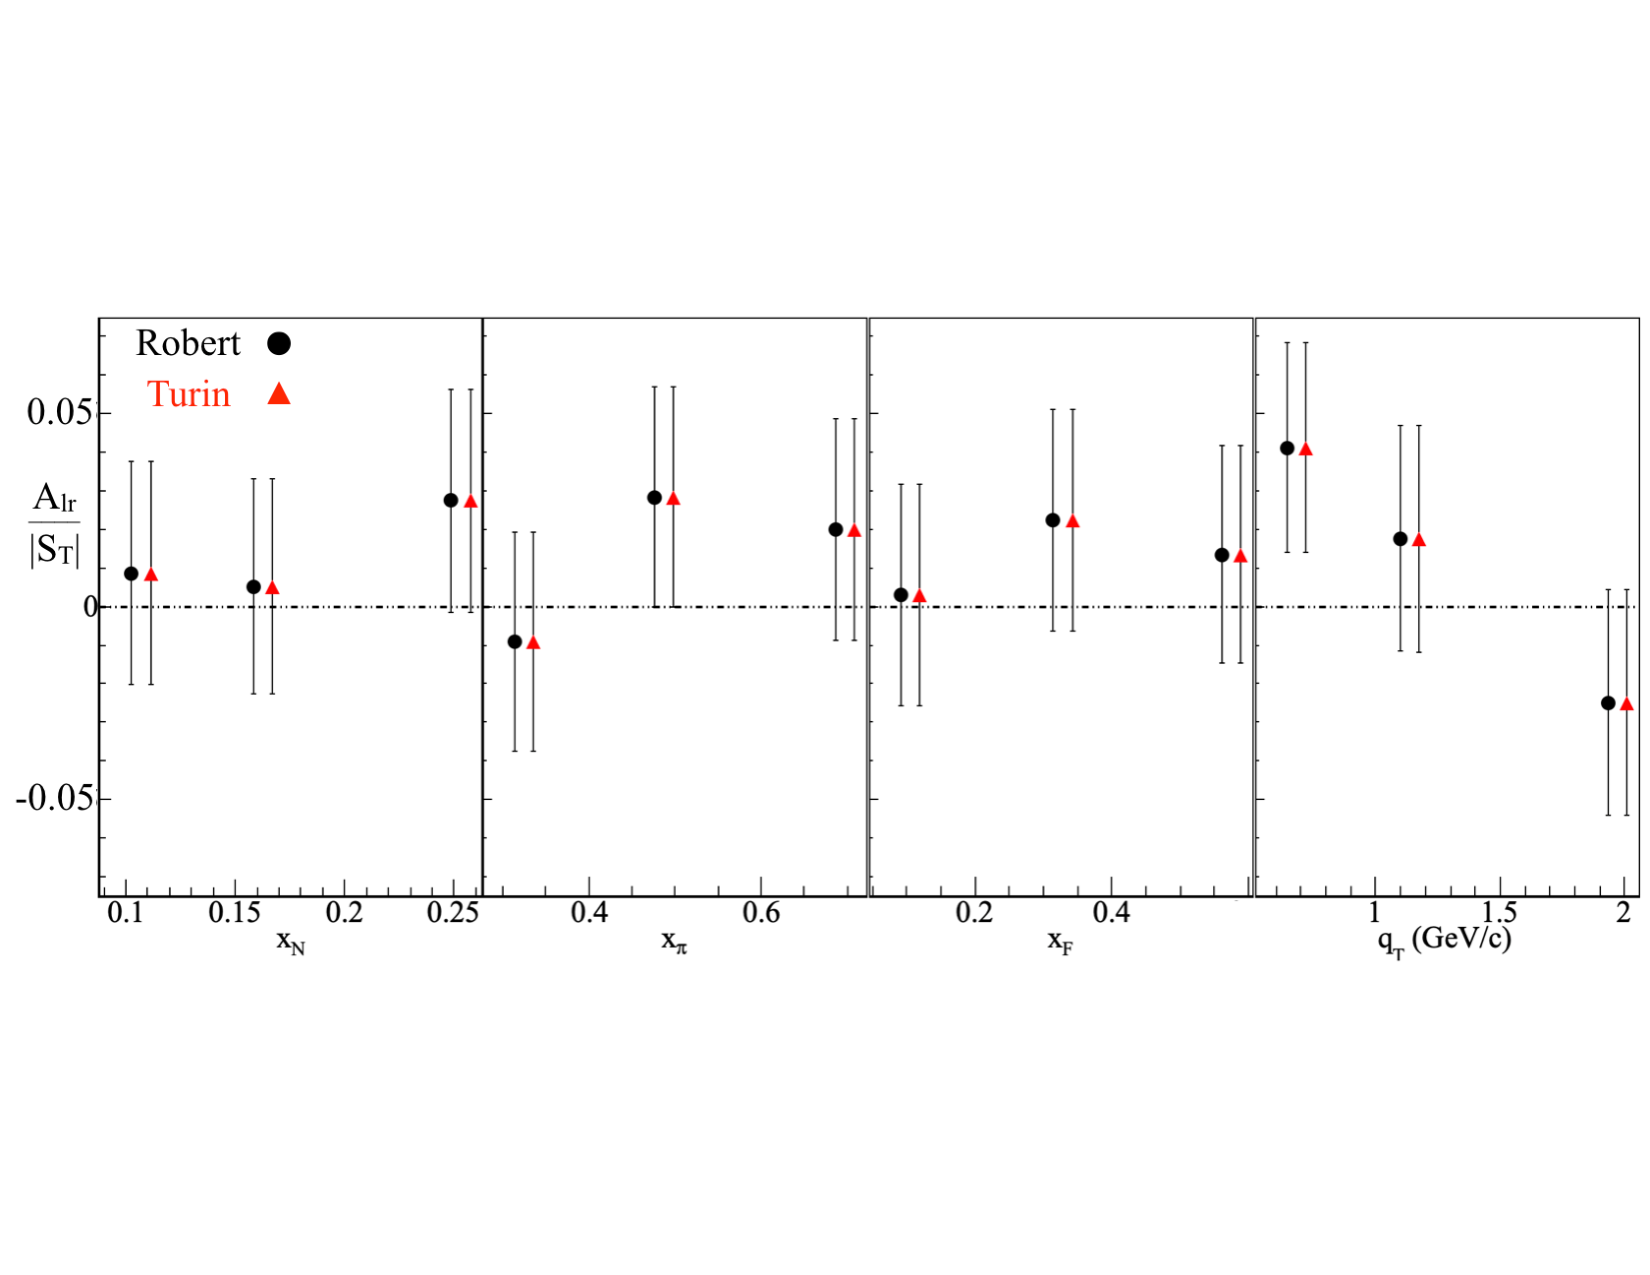
\includegraphics[width=\textwidth,trim=0cm 5cm 0cm 5cm,clip]{Alr_xCheck}
  \caption{The left-right asymmetry without corrections for polarization or
    dilution factor from the W07 period.  The values from this thesis are the
    black circles and the cross-check values are the red triangles.}
  \label{fig::Alr_xCheck}
\end{figure}

